

\documentclass[a4paper,12pt,spanish]{article}

\usepackage[utf8]{inputenc}


\usepackage{blindtext}
%\usepackage{microtype}
\usepackage{amsfonts, amsmath, amsthm, amssymb}
%\usepackage{fancyhdr}
%\usepackage{index}
%\usepackage{multicol}    

\usepackage[T1]{fontenc}
\usepackage[utf8]{inputenc}
\usepackage{graphicx}
\usepackage[spanish,es-tabla]{babel}
\usepackage{url}
\usepackage{enumitem}

\usepackage[unicode=true, pdfusetitle,
bookmarks=true,bookmarksnumbered=false,bookmarksopen=false,
breaklinks=true,pdfborder={0 0 1},backref=false,colorlinks=false]
{hyperref}

\usepackage{listings}


\usepackage{siunitx} %para el sistema internacional
\usepackage[export]{adjustbox}
\usepackage{booktabs} 
\usepackage{subcaption}

\usepackage{float}


\newcommand{\address}[1]{
	\par {\raggedright #1
		\vspace{1.4em}
		\noindent\par}
}


\pagenumbering{gobble}
\include{noNumberPage}
\pagenumbering{arabic}
\setcounter{page}{62}

%tutorial de tablas latex: https://manualdelatex.com/tutoriales/tablas

\usepackage{multirow}

% \usepackage[table,xcdraw]{xcolor}


%Inicio del documento (hasta que se cierre con \end{document}
\begin{document}





\title{El diodo}

%\author{Adrián Rivero Fernández}
\date{}

\maketitle



\begin{abstract} %resumen

En esta práctica analizaremos un diodo y un diodo Zener. En el caso del diodo, dibujaremos la curva característica y construiremos un circuito limitador. Para el Zener, determinaremos sus características y su capacidad de regulación.

%INDICAR CUALES CARACTERÍSTICAS


\end{abstract}




\section{Material y métodos}

Utilizaremos un generador de funciones, un polímetro, un osciloscopio de doble canal, una placa de prototipo (\textit{protoboard}) donde montaremos el circuito, distintas resistencias comerciales de distintos valores, diodos de pequeña señal D1N4148 o D1N4007, un diodo zener BZX85 C4V7 de 1,3 W, y una fuente de alimentación variable de corriente contínua.

La práctica se divide en dos partes. 

\subsection{Diodo en pequeña señal}

En la primera analizaremos las características del diodo de pequeña señal, utilizando el circuito de la Figura 1.

\begin{figure}[H]
	\centering
	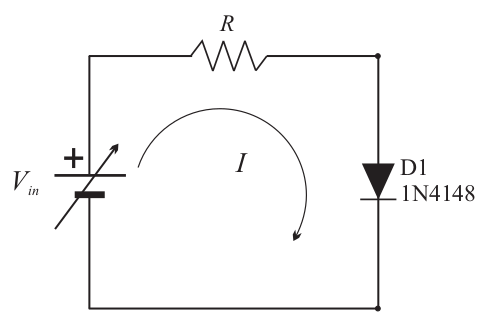
\includegraphics[width=0.6\linewidth]{circuito}
	\caption{Circuito de prueba del diodo}
	\label{fig:circuito}
\end{figure}

\subsection*{Curva característica}

Mediante la hoja de características determinaremos el valor mínimo de R para el caso más desfavorable de tensión, y montaremos el circuito con una resistencia de más del doble de ese valor.

Luego realizaremos un barrido en continua desde -10 V hasta +10 V. Mediremos el voltaje de entrada en los bornes del diodo, $V_D$, y la caída de tensión en la resistencia de protección, $V_R$.

Calcularemos la corriente y representaremos gráficamente la corriente de la resistencia en función de $V_D$ para ambas polarizaciones.

\subsection*{Circuito limitador}

El circuito limitador permite eliminar tensiones no deseadas en la carga.

Usaremos el circuito de la Figura 2, aplicando una señal sinusoidal de amplitud 10 V y con una frecuencia de 1 kHz.


\begin{figure}[H]
	\centering
	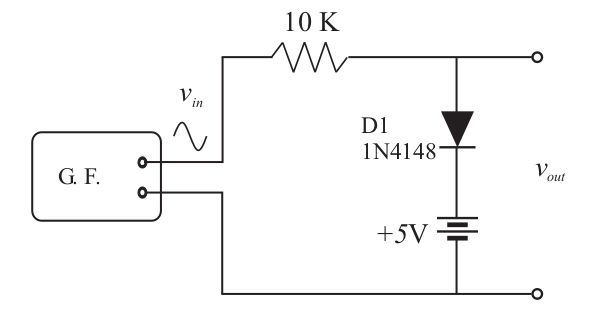
\includegraphics[width=0.6\linewidth]{circuito2}
	\caption{Circuito limitador}
	\label{fig:circuito2}
\end{figure}

\subsection{Diodo zener}

\subsection*{Características}

Montaremos el circuito de prueba para el diodo zener de la Figura 3, con una resistencia de protección de alrededor de 100$\si{\ohm}$

Realizaremos un barrido en contínua desde 0V hasta $V_{max}$. Mediremos la caida de tensión en los bornes de la resistencia de protección y en los bordnes del diodo zener, $V_R$ y $V_z$.


\begin{figure}[H]
	\centering
	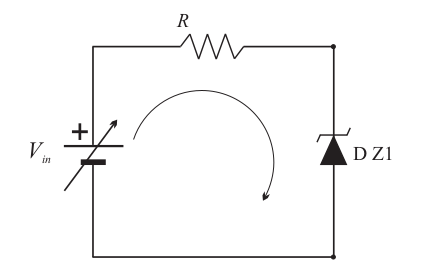
\includegraphics[width=0.6\linewidth]{circuito5}
	\caption{circuito de prueba del diodo zener}
	\label{fig:circuito5}
\end{figure}

\subsection*{Capacidad de regulación}

Montamos el circuito de la Figura 4 con $V_{in}= 10\si{V}$ y siendo $R_L$ la caja de resistencias. Haremos un barrido sobre $R_L$ desde 9kW hasta 100W.

\begin{figure}[H]
	\centering
	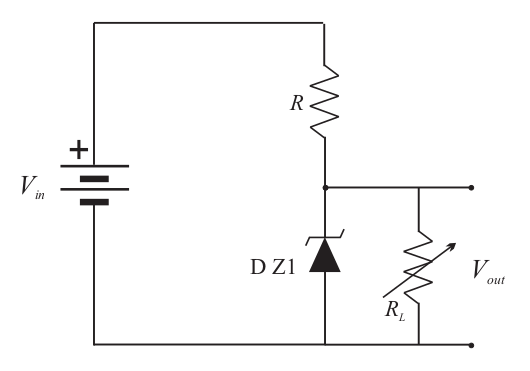
\includegraphics[width=0.6\linewidth]{circuito6}
	\caption{Circuito de prueba de carga}
	\label{fig:circuito6}
\end{figure}




\section{Resultados y discusión}


\subsection{Diodo en pequeña señal}

\subsection*{Curva característica}

La tensión más desfavorable es 10V, la intensidad máxima es 1A, y el voltaje correspondiente 1,1V. De modo que 
\[ 10 - 1,1 = 8,9 \si{V} \]
De aquí determinamos que la intensidad mínima es 
\[R_{min}= 8,2 \si{\ohm}\]

Nosotros instalaremos una resistencia de $510\si{\ohm}$, por comodidad para la toma de medidas.

Sin embargo, para la polarización inversa tomaremos una resistencia del orden de los $\si{\mega \ohm}$, por comodidad para apreciar las medidas.

En la Tabla 1 tenemos el barrido realizado.

\begin{table}[H]
	\centering
	\begin{tabular}{|l|l|l|l|}
		\hline
		$V_{in}$ (V) & $V_D$ (V) & $V_R$ (V)    & $I $(A)    \\ \hline
		-20 & 20  $\pm 1$     & 0,0005 $\pm 0,0001$ & (9,80$\pm2$)E-07 \\ \hline
		-15 & 15 $\pm 1$      & 0,00028$\pm 0,0001$ & (5,50$\pm2$)E-07 \\ \hline
		-10 & 10 $\pm 1$      & 0,00013$\pm 0,0001$ & (2,55$\pm2$)E-07 \\ \hline
		-8  & 8  $\pm 1$      & (8$\pm1$)E-05  	    & (1,57$\pm2$)E-07 \\ \hline
		-6  & 6  $\pm 1$      & (3$\pm1$)E-05       & (5,88$\pm2$)E-08 \\ \hline
		-4  & 4  $\pm 1$      & (1$\pm1$)E-05 	    & (1,96$\pm2$)E-08 \\ \hline
		-2  & 2  $\pm 1$      & (1$\pm1$)E-05	    & (1,96$\pm2$)E-08   \\ \hline
		0,3 & 0,287 $\pm 0,001$    & 0,0002 $\pm 0,0001$  & 3,92E-07$\pm2$E-07 \\ \hline
		0,6 & 0,512 $\pm 0,001$    & 0,1222$\pm 0,0001$  & 0,00024  $\pm7$E-07 \\ \hline
		1   & 0,571   $\pm 0,001$  & 0,470  $\pm 0,001$  & 0,00092  $\pm4$E-06 \\ \hline
		2   & 0,619   $\pm 0,001$  & 1,414  $\pm 0,001$ & 0,0028    $\pm7$E-06 \\ \hline
		3   & 0,643  $\pm 0,001$   & 2,388 $\pm 0,001$  & 0,0047    $\pm1$E-05 \\ \hline
		4   & 0,659  $\pm 0,001$   & 3,348$\pm 0,001$   & 0,006     $\pm2$E-05 \\ \hline
		5   & 0,670  $\pm 0,001$   & 4,32 $\pm 0,01$   & 0,0085     $\pm4$E-05 \\ \hline
		6   & 0,679 $\pm 0,001$    & 5,25 $\pm 0,01$   & 0,010      $\pm4$E-05 \\ \hline
		7   & 0,686  $\pm 0,001$   & 6,27 $\pm 0,01$   & 0,012      $\pm4$E-05  \\ \hline
		8   & 0,693 $\pm 0,001$    & 7,25 $\pm 0,01$   & 0,014      $\pm5$E-05 \\ \hline
		9   & 0,699  $\pm 0,001$   & 8,27 $\pm 0,01$   & 0,016      $\pm5$E-05\\ \hline
		10  & 0,703  $\pm 0,001$   & 9,28 $\pm 0,01$   & 0,018      $\pm6$E-05 \\ \hline
	\end{tabular}  
	\caption{Medidas del diodo en pequeña señal}
	\label{tab:my-table}
\end{table}

En la Figura 5 tenemos representada la corriente de la resistencia en función del voltaje $V_D$ para polarización directa, con el ajuste de la curva, y en la Figura 6 para polarización inversa.

\begin{figure}[H]
	\centering
	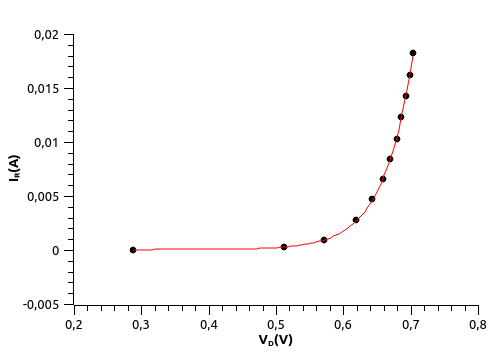
\includegraphics[width=0.75\linewidth]{grafica1}
	\caption{Corriente por la resistencia en función del $V_D$ para polarización directa}
	\label{fig:grafica1}
\end{figure}

%A=1.88546223539708e-09
%t=-0.0437523387795083
%y0=4.34744192475465e-05

%y0+A*exp(-x/t)
Siendo el ajuste exponencial:
\[4,347 + 1,885 e^{\frac{-x}{-0,044}}\]

\begin{figure}[H]
	\centering
	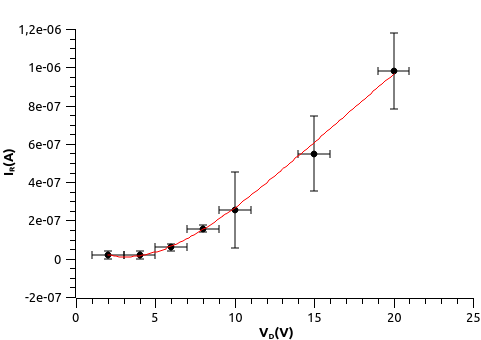
\includegraphics[width=0.75\linewidth]{grafica2}
	\caption{Corriente por la resistencia en función del $V_D$ para polarización inversa}
	\label{fig:grafica2}
\end{figure}

%A1=0.0905803991286812
%t1=35.0440696343226
%A2=-0.0905906222067738
%t2=35.0482675230202
%y0=1.02533199007862e-05

%A1*exp(-x/t1)+A2*exp(-x/t2)+y0


Siendo el ajuste exponencial:
\[0,091 e^{\frac{-x}{35,04}}- 0,091 e^{\frac{-x}{35,05}+ 1,025}\]


Para un valor típico de $V_R = -7 \si{V}$, vemos con la gráfica que 
\[\boxed{I_{Rmax} = $1,2E-07$  \si{A} } \]

Utilizando la curva ajustada en la Figura 5, vemos que para 1 mA la tensión de codo es 
\[ \boxed{V_g = 0,6 \si{V}}
\]

Suponiendo $\eta = 1$, la resistencia dinámica es ($r_d = \frac{25\eta}{I(\si{mA})}$)

\[r_d (1,5 \si{mA}) = 16,67 \si{\ohm} \]
\[r_d (10  \si{mA}) = 2,5 \si{\ohm} \]

\subsection*{Circuito limitador}

Suponiendo que el diodo es ideal, la forma del voltaje de salida $v_{out}= v_{out}(t)$ y la curva de transferencia $v_{out} = v_{out}(v_{in})$ tienen las formas presentadas en las Figuras 7 y 8 respectivamente. Vemos que el circuito corta el voltaje en 5V.

En las Figuras 9 y 10 tenemos el voltaje de salida y la curva de transferencia de nuestro montaje experimental.

Vemos que presentan una ligera diferencia, en los bordes presentan unas pequeñas desviaciones, ampliadas en las Figuras 11 y 12. Estas imperfecciones se manifiestan debido a que, dado que el diodo no es ideal, actúa ligeramente como capacitor en esos puntos.

\begin{figure}[H]
	\centering
	\includegraphics[width=0.7\linewidth]{"../fotos/voltaje a mano"}
	\caption{voltaje de salida en el circuito limitador de +5V}
	\label{fig:voltaje-a-mano}
\end{figure}

\begin{figure}[H]
	\centering
	\includegraphics[width=0.7\linewidth]{"../fotos/curva de transferencia a mano"}
	\caption{curva de transferencia del circuito limitador de +5V}
	\label{fig:curva-de-transferencia-a-mano}
\end{figure}


\begin{figure}[H]
	\centering
	\includegraphics[width=0.7\linewidth]{"../fotos/voltaje experimental"}
	\caption{Voltaje del montaje experimental del limitador de +5V}
	\label{fig:voltaje-experimental}
\end{figure}

\begin{figure}[H]
	\centering
	\includegraphics[width=0.7\linewidth]{"../fotos/curva transferencia experimental"}
	\caption{Curva de transferencia del montaje experimental del limitador de +5V}
	\label{fig:curva-transferencia-experimental}
\end{figure}

\begin{figure}[H]
	\centering
	\includegraphics[width=0.7\linewidth]{"../fotos/imperfeccion en voltaje"}
	\caption{Imperfecciones en la curva del voltaje de salida}
	\label{fig:imperfeccion-en-voltaje}
\end{figure}

\begin{figure}[H]
	\centering
	\includegraphics[width=0.7\linewidth]{"../fotos/imperfeccion en transferencia"}
	\caption{Imperfecciones en la curva de transferencia}
	\label{fig:imperfeccion-en-transferencia}
\end{figure}



En caso de querer construir un circuito limitador para voltajes negativos, debemos cambiar el sentido del diodo de modo que el montaje quede como el de la Figura 13.

Podemos ver en las Figuras 14 y 15 el voltaje y la curva de transferencia.

\begin{figure}[H]
	\centering
	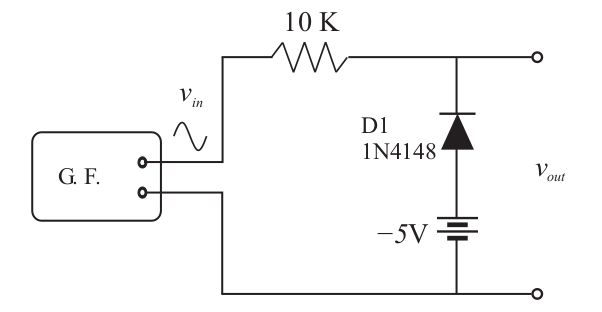
\includegraphics[width=0.6\linewidth]{circuito3}
	\caption{Circuito limitador a -5V}
	\label{fig:circuito3}
\end{figure}



\begin{figure}[H]
	\centering
	\includegraphics[width=0.7\linewidth]{"../fotos/voltaje lim negativo"}
	\caption{voltaje del limitador de -5V}
	\label{fig:voltaje-lim-negativo}
\end{figure}

\begin{figure}[H]
	\centering
	\includegraphics[width=0.7\linewidth]{"../fotos/transf lim negativo"}
	\caption{función de transferencia del limitador a -5V}
	\label{fig:transf-lim-negativo}
\end{figure}

Para construir un limitador que proporcione una señal cuadrada de $\pm 5 \si{V}$, hay que construir el circuito de la Figura 16, y se obtienen el voltaje y la curva de transferencia de las Figuras 17 y 18.

\begin{figure}[H]
	\centering
	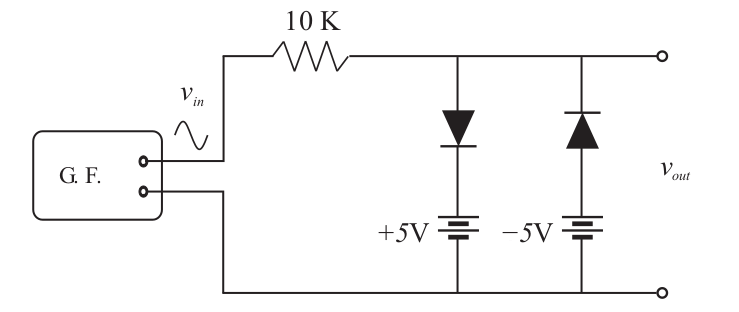
\includegraphics[width=0.6\linewidth]{circuito4}
	\caption{circuito limitador para señal cuadrada de $\pm 5 \si{V}$}
	\label{fig:circuito4}
\end{figure}

\begin{figure}[H]
	\centering
	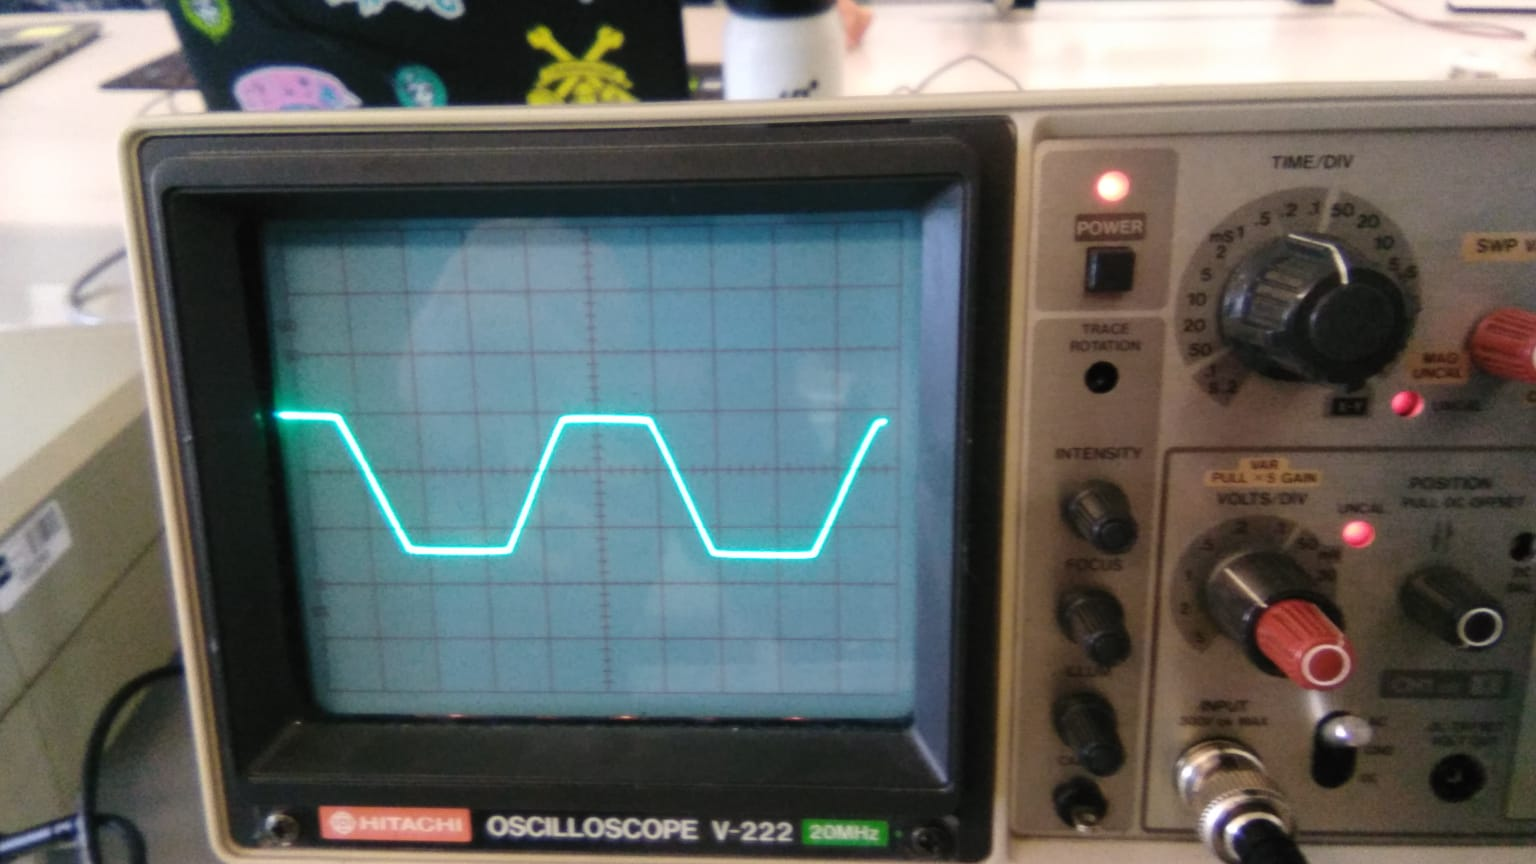
\includegraphics[width=0.7\linewidth]{../fotos/cuadrada}
	\caption{voltaje del circuito limitador de onda cuadrada}
	\label{fig:cuadrada}
\end{figure}

\begin{figure}[H]
	\centering
	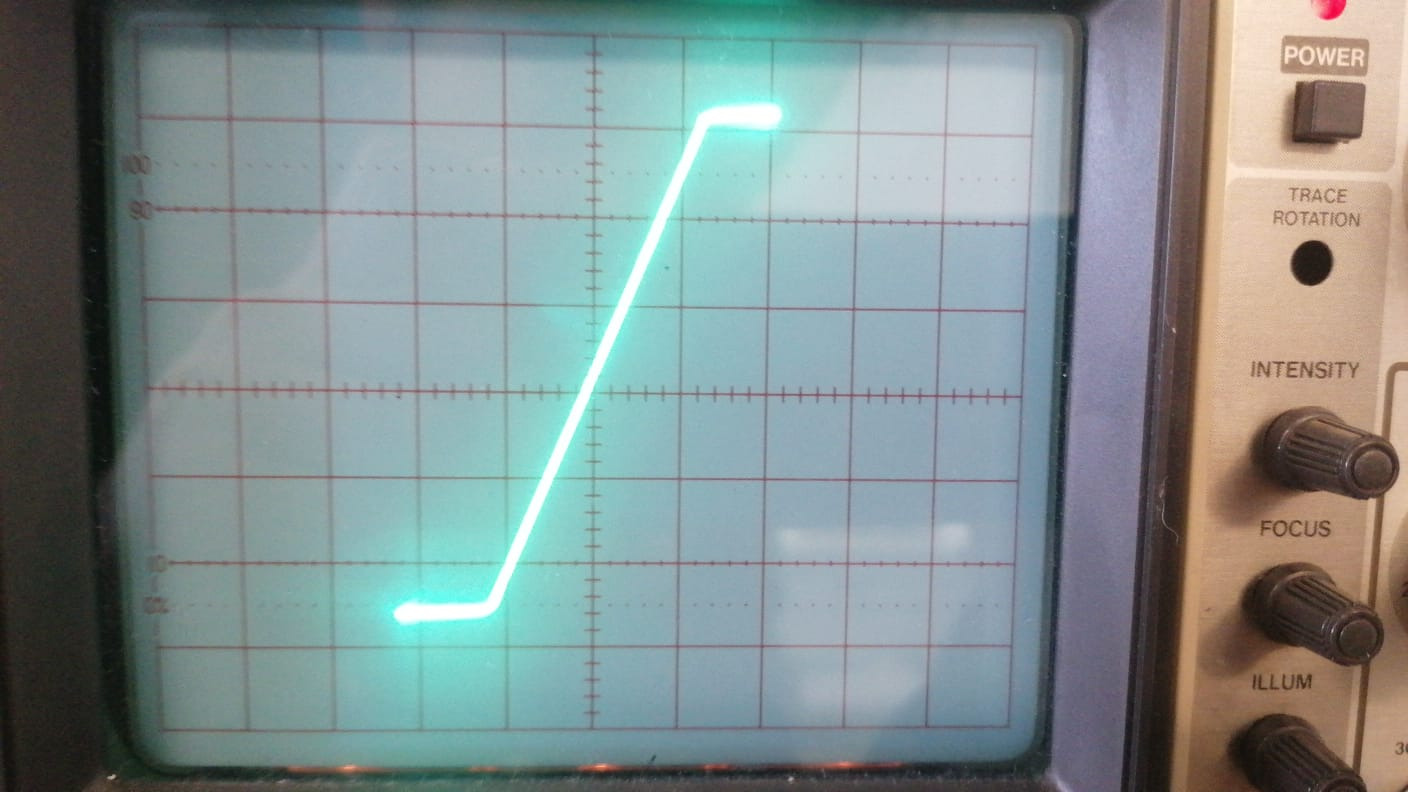
\includegraphics[width=0.7\linewidth]{../fotos/cuadrada-transf}
	\caption{función de transferencia del circuito limitador de onda cuadrada}
	\label{fig:cuadrada-transf}
\end{figure}

\begin{figure}[H]
	\centering
	\includegraphics[width=0.7\linewidth]{"../fotos/montaje experimental"}
	\caption{Montaje del circuito limitador}
	\label{fig:montaje-experimental}
\end{figure}



\subsection{Diodo zener}

Los resultados obtenidos del circuito con el zener están representados en la Tabla 2.

\begin{table}[H]
	\centering
	\begin{tabular}{|c|l|l|l|}
		\hline
		$V_{in}$ (V) & $V_Z$ (V) & $V_R$ (V)  & $I$ (A)   \\ \hline
		0   & 0,05 $\pm 0,01$   & 0     $\pm 0,01$ & 0   $\pm 0,0001  $    \\ \hline
		1   & 1,1  $\pm 0,01$    & 0    $\pm 0,01$ & 0      $\pm 0,0001  $ \\ \hline
		2   & 2,1  $\pm 0,01$    & 0,013$\pm 0,01$ & 0,00013$\pm 0,0001  $ \\ \hline
		3   & 2,9  $\pm 0,01$    & 0,03 $\pm 0,01$ & 0,0003 $\pm 0,0001  $ \\ \hline
		4   & 3,7  $\pm 0,01$    & 0,28 $\pm 0,01$ & 0,00283$\pm 0,00013  $ \\ \hline
		5   & 4,13 $\pm 0,01$    & 0,8  $\pm 0,01$ & 0,008  $\pm 0,00018  $ \\ \hline
		6   & 4,36 $\pm 0,01$    & 1,62 $\pm 0,01$ & 0,0162 $\pm 0,0003  $ \\ \hline
		7   & 4,46 $\pm 0,01$    & 2,54 $\pm 0,01$ & 0,0254 $\pm 0,0004  $ \\ \hline
		8   & 4,54 $\pm 0,01$    & 3,42 $\pm 0,01$ & 0,0342 $\pm 0,0004  $ \\ \hline
		9   & 4,61 $\pm 0,01$    & 4,43 $\pm 0,01$ & 0,0443 $\pm 0,0005  $ \\ \hline
		10  & 4,64 $\pm 0,01$    & 5,34 $\pm 0,01$ & 0,0534 $\pm 0,0006  $ \\ \hline
		11  & 4,56 $\pm 0,01$    & 6,31 $\pm 0,01$ & 0,0631 $\pm 0,0007  $ \\ \hline
		12  & 4,7  $\pm 0,01$    & 7,26 $\pm 0,01$ & 0,0726 $\pm 0,0008  $ \\ \hline
	\end{tabular}
	\caption{Resultados para el circuito de prueba del zener}
	\label{tab:my-table}
\end{table}



En la Figura 20 está representada la corriente en función del voltaje zener.

\begin{figure}[H]
	\centering
	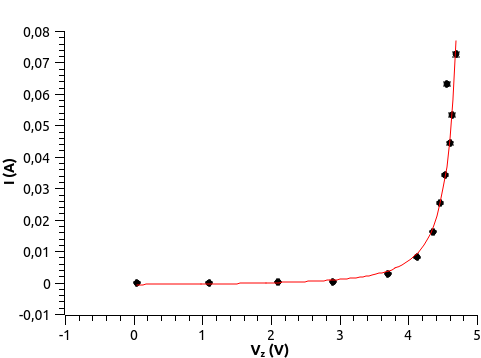
\includegraphics[width=0.7\linewidth]{grafica3}
	\caption{Corriente en función del voltaje del zener}
	\label{fig:grafica3}
\end{figure}

%A=6.10202125515459
%xc=4.78125888736549
%w=0.493400815127149
%y0=-0.0961920923454529

%y0+2*A/PI*w/(4*(x-xc)^2+w^2)
Siendo el ajuste exponencial:
%\[-0.096 + \frac{2A}{\pi}\frac{w}{4(x-x_c)^2+w^2}\]
\[-0.096 + \frac{2\cdot6.102}{\pi}\frac{0.49}{4(x-4.78)^2+0.49^2}\]


Según la gráfica, podemos determinar los valores de la tensión del zener para las siguientes intensidades:
\begin{itemize}
	\item $V_Z (15\si{mA}) = 2,3\si{V}$
	\item $V_Z (20\si{mA}) = 2,5\si{V}$
	\item $V_Z (25\si{mA}) = 2,8\si{V}$
\end{itemize}

Para calcular la impedancia del zener al pasar 20mA de corriente, podemos utilizar dos puntos de la tabla anterior:
\[ Z_{zener} = \frac{\Delta V}{\Delta I} = \frac{4,46- 4,36}{0,0254 - 0,0162} = 10,87 \si{\ohm} \]

\subsection*{Capacidad de regulación de un diodo zener}

La Tabla 3 contiene el barrido sobre $R_L$ del circuito de prueba de carga. 


\begin{table}[H]
	\centering
	\begin{tabular}{|ll|}
		\hline
		\multicolumn{2}{|c|}{$V_{in} = 10$ V}         \\ \hline
		\multicolumn{1}{|l|}{$R_L (\si{k\ohm})$} & $V_{out} (\si{V})$ \\ \hline
		\multicolumn{1}{|l|}{9$\pm 0,01$}           & 4,63 $\pm 0,01$  \\ \hline
		\multicolumn{1}{|l|}{7$\pm 0,01$}           & 4,63$\pm 0,01$   \\ \hline
		\multicolumn{1}{|l|}{5$\pm 0,01$}           & 4,62 $\pm 0,01$  \\ \hline
		\multicolumn{1}{|l|}{3$\pm 0,01$}           & 4,62 $\pm 0,01$  \\ \hline
		\multicolumn{1}{|l|}{1$\pm 0,01$}           & 4,62 $\pm 0,01$  \\ \hline
		\multicolumn{1}{|l|}{0,8$\pm 0,01$}         & 4,61 $\pm 0,01$  \\ \hline
		\multicolumn{1}{|l|}{0,6$\pm 0,01$}         & 4,6 $\pm 0,01$   \\ \hline
		\multicolumn{1}{|l|}{0,5$\pm 0,01$}         & 4,59$\pm 0,01$   \\ \hline
		\multicolumn{1}{|l|}{0,4$\pm 0,01$}         & 4,58$\pm 0,01$   \\ \hline
		\multicolumn{1}{|l|}{0,3$\pm 0,01$}         & 4,56$\pm 0,01$   \\ \hline
		\multicolumn{1}{|l|}{0,25$\pm 0,01$}        & 4,54$\pm 0,01$   \\ \hline
		\multicolumn{1}{|l|}{0,2$\pm 0,01$}         & 4,51$\pm 0,01$   \\ \hline
		\multicolumn{1}{|l|}{0,15$\pm 0,01$}        & 4,45 $\pm 0,01$  \\ \hline
		\multicolumn{1}{|l|}{0,1$\pm 0,01$}         & 4,27 $\pm 0,01$  \\ \hline
	\end{tabular}
	\caption{Resultados para el circuito de prueba de carga}
	\label{tab:my-table}
\end{table}

Podemos ver que el zener deja de regular para el valor de resistencia de carga 
\[R_L = 0,1 \si{k\ohm}\]

donde la tensión cae un 5\%

Se puede observar también en la Figura 21, que representa gráficamente la Tabla 3.

\begin{figure}[H]
	\centering
	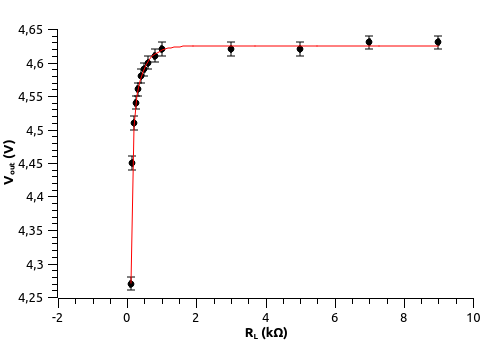
\includegraphics[width=0.7\linewidth]{grafica_ultima}
	\caption{Tensión de salida en función de la resistencia de carga}
	\label{fig:graficaultima}
\end{figure}


%A1=0.00235783731566995
%t1=-4.98990633163981
%A2=-0.200534887845527
%t2=0.250339313763709
%A3=-2.72918833118251
%t3=0.0393175851713483
%y0=4.61674768473672

%A1*exp(-x/t1)+A2*exp(-x/t2)+A3*exp(-x/t3)+y0
Siendo el ajuste exponencial:
\[ 0,002 e^{\frac{-x}{-4,99}}-0,2e^{\frac{-x}{0,25}}-2,73 e^{\frac{-x}{0,04}}+4,617
\]





%%%%%%%%%%%%%%%%%%%%%%%%%%%
\begin{thebibliography}{1}
%%%%%%%%%%%%%%%%%%%%%%%%%%%
	
	
	\bibitem{UNED2022} (varios) Guiones de prácticas- Técnicas Experimentales II. Grado en Física. Versión 2.1  UNED, 2022 \url{https://2022.cursosvirtuales.uned.es/o/3754218}
	%	\bibitem{UNED2021} (varios) Técnicas Experimentales I. Versión 3.5.  UNED, 2021 \url{https://2021.cursosvirtuales.uned.es/o/42035617}
	%\bibitem{2021} Densidad de materiales \url{ https://www.stemm.com/index.php/es/densidades-de-materiales }
	
	
\end{thebibliography}

\end{document}